\chapter{Componentes mecánicos}

Una vez determinado los componentes electrónicos necesarios para el correcto funcionamiento del brazo robótico es necesario determinar los componentes mecánicos.

\section{Actuador}

Una de las partes mecánicas más importantes es el actuador, es decir, el mecanismo que proporcionará la fuerza necesaria para mover las articulaciones del robot.

Para la correcta selección o desarrollo del actuador necesitamos dos parámetros que vimos en los capítulos anteriores, el primero es el torque necesario para realizar los desplazamientos del robot a la velocidades y aceleraciones requeridas y el segundo es la velocidad nominal del motor a utilizar.

Por norma general, los motores eléctricos y, para nuestro caso, los motores eléctricos sin escobillas, funcionan a velocidades altas y un torque relativamente pequeño, para esto es necesario utilizar reductores de velocidad, los cuales cumplen dos objetivos primordiales: reducir la velocidad en eje de salida y aumentar el torque en el mismo.

El siguiente paso es escoger un reductor de velocidad que cumpla con los requerimientos específicos de nuestro brazo robótico, los cuales son:

\begin{itemize}
\item Alta relación de transmisión, mayor a 10:1.
\item Precisión, necesaria para realizar los movimientos deseados sin demasiado juego. 
\item Efectividad de transmisión, necesaria para no perder demasiada energía
\end{itemize}

Estos son algunos de los más importantes, existen otros factores a considerar como el tamaño final del reductor y la facilidad de manufactura.

Para el desarrollo de este brazo robótico se han considerado tres diferentes tipos de reductores de velocidad, cada uno con ventajas y desventajas que se mencionarán a continuación.

\subsection{Engranes planetarios}

El primero en esta lista es un reductor con engranes planetarios, 

Existen proyectos como el de [insertar cita despúes] OpenTorque Actuator de Gabrael Levine que utiliza engranes planetarios en el diseño de su actuador, logra una relación de transmisión de 8:1

En la imagen \ref{fig:opentorque} podemos apreciar su diseño con engranes planetarios del tipo  helicoidal así como una carcasa para el sistema de motor y actuador. 

\begin{figure}[h]
    \centering
    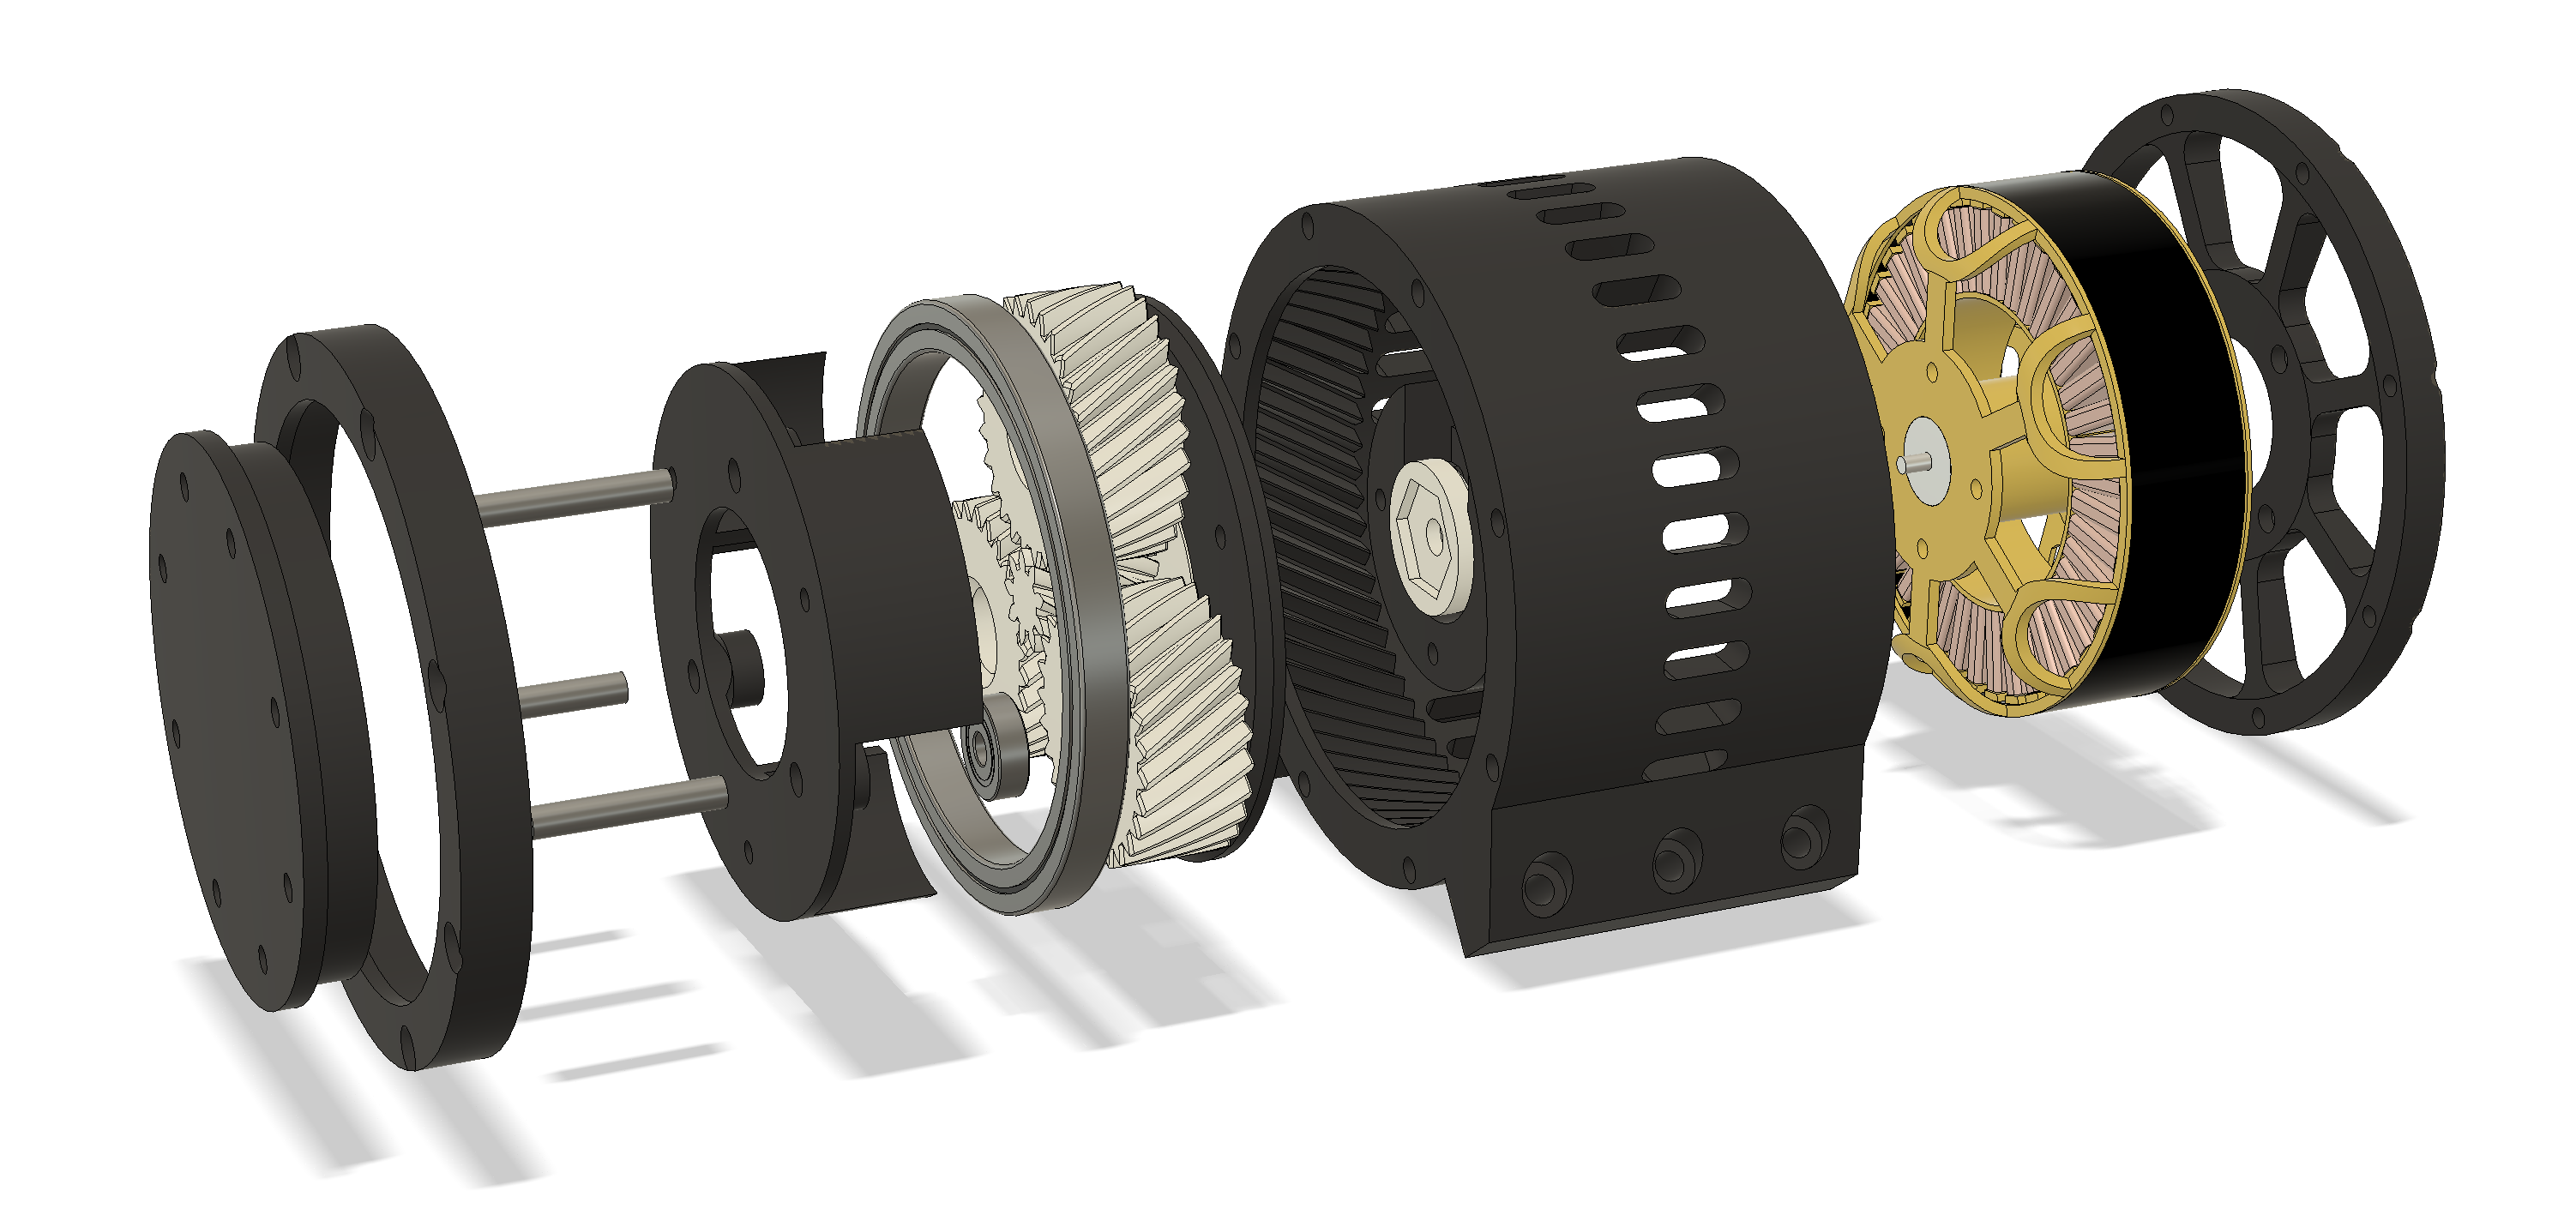
\includegraphics[width=15cm, height=6cm, keepaspectratio]{./img/chapter6/opentorque.png}
    \caption{OpenTorque Actuator por Gabrael Levine}
    \label{fig:opentorque}
\end{figure}

En esta propuesta la ventaja es la relativa facilidad de fabricación con tecnología de manufactura aditiva así como un tamaño y peso considerablemente pequeño.

Las desventajas son su relativamente pequeño relación de transmisión y su poca eficiencia de transmisión.

\subsection{Engrane cicloidal}
\subsection{Harmonic Drive}
